\documentclass[12pt]{exam}

\usepackage{amssymb}
\usepackage{mathtools}
\usepackage{algorithm}
\usepackage{float}  % Figure placement
\usepackage{minted}  % Code highlighting
\usepackage{tikz}  % Flow chart
\usepackage{lipsum}
\usepackage{xspace}
\usepackage{hyperref}
\usepackage{MnSymbol}
\usepackage{pgffor}


\hypersetup{
    colorlinks = true,
    linkcolor = blue,
    urlcolor  = blue,
    citecolor = blue,
    anchorcolor = blue
}

\newcommand{\hwheaderfooter}[3]{
\pagestyle{headandfoot}
\firstpageheadrule
\firstpageheader{#1}{#2}{#3}
\runningheader{#1}{#2}{#3}
\runningheadrule
\firstpagefooter{}{\thepage}{}
\runningfooter{}{\thepage}{}
}

\newcommand{\latex}{\LaTeX\xspace}

\newcommand{\stars}[1]{%
    \foreach \n in {1,...,#1}{%
        $\filledstar$%
    }%
}

\hwheaderfooter{HW 4}{Ching}{CSCI 406}


\begin{document}
\begin{center}
    \fbox{\fbox{\parbox{\textwidth - 0.2 in}{\centering

                {Instructions: Please note that handwritten assignments \textbf{will not be graded}. Use the
                    provided \latex template to complete your homework. Please do not alter the order or spacing of
                    questions (keep each question on its own page). When you submit to Gradescope, you must mark
                    which page(s) correspond to each question. \textbf{You may not receive credit for unmarked
                        questions}. \\ When including graphical figures, we encourage the use of tools such as \href{https://dreampuf.github.io/GraphvizOnline/}{graphviz} or packages like \href{https://www.overleaf.com/learn/latex/TikZ_package}{tikz} for simple and complex figures. However, these may be handwritten only if they are neat and legible (as defined by the grader). }\\

            }}}
\end{center}

\textbf{List any collaborators (besides TAs or professors) here:}

\begin{questions}

    \question[35] [W4, \stars{5}] Alternative Topological Sorting

    When topologically sorting a directed-acyclic graph (DAG), let any edge $A \to B$ denote that $A$ must come before $B$ in any valid topological ordering.

    From the last homework, you know that a topological order must start with a vertex that has no incoming edges (in-degree of zero).
    \begin{parts}
        \part[10] Prove that a directed-acyclic graph has at least one vertex with in-degree zero and one vertex with out-degree zero. (Hint: prove in-degree by contradiction, and then reference that proof for out-degree).

        \textbf{Proof by contradiction:} Assume that a DAG has no vertex with in-degree zero. Then, there is no vertex that can be the first vertex in a topological ordering. This contradicts the definition of a topological ordering. Therefore, a DAG must have at least one vertex with in-degree zero.

        For the out-degree, the proof is the same as above but with the roles of in-degree and out-degree reversed.

        \part[15] Based on your previous answer, describe an algorithm for topological sorting that uses in-degrees to process vertices. The complexity of your algorithm must be no worse than the DFS-based toposort algorithm discussed in class.

        \begin{enumerate}
            \item Create an array to store the in-degree of each vertex.
            \item Enqueue all vertices with in-degree zero.
            \item While the queue is not empty, do the following:
                  \begin{itemize}
                      \item Dequeue a vertex $v$ from the queue.
                      \item Add $v$ to the topological ordering.
                      \item For each neighbor $u$ of $v$, decrement the in-degree of $u$ by one.
                      \item If the in-degree of $u$ is zero, enqueue $u$.
                  \end{itemize}
            \item If the topological ordering contains all vertices, return the topological ordering. Otherwise, return that the graph has a cycle.

        \end{enumerate}


        \part[10] While running this algorithm, it reaches a point where there are still vertices left that have not been processed, yet none of these vertices have an in-degree of zero. What does this indicate about the graph?

        This indicates that the graph contains a cycle.


    \end{parts}

    \clearpage


    \question[10] [W5, \stars{2}] MST.

    \begin{parts}
        \part[2] Select whether the statement is true or false,
        and write a \textit{brief} explanation of your reasoning.

        If each edge of a graph has a unique weight, the MST of that graph will be unique.

        % Replace \square with \blacksquare for the option you would like to select.
        $\blacksquare$ True $\square$ False
        \hspace{0.5in} \textbf{No explanation necessary for part (a).}

        \part[4] Describe how you would modify Prim's algorithm to compute the \textbf{maximum} spanning tree. (That is, the tree with the highest cost.)

        Simply change the edge selection criteria from the minimum to the maximum.

        \part[4] Describe how you would modify Kruskal's algorithm to compute the \textbf{maximum} spanning tree. (That is, the tree with the highest cost.)

        Change the sorting order of the edges from ascending to descending.

    \end{parts}
    \clearpage

    \question[10] [W5, \stars{1}] Disjoint Set Data Structure.

    \vspace*{-0.2cm}
    \begin{figure}[h]
        \center
        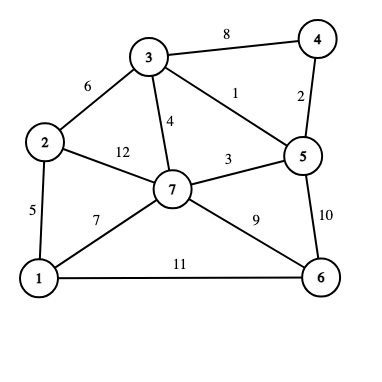
\includegraphics[width = 3in]{hw4-q3.png}
    \end{figure}

    \vspace*{-1.5cm}

    Run the Kruskal's algorithm on the graph above and show the state of the disjoint set array each time after an edge is added to the MST. Do not use path compression and attach the smaller component to the larger component during merge. {\bf When merging components of same sizes, attach the component with the smaller root node ID to the larger one. See I1 below.} You can track component sizes manually (no need to show sizes in your solution).

    \par{{\bf I0:}
        \begin{tabular}{|c|c|c|c|c|c|c|}
            \multicolumn{1}{c}{1} & \multicolumn{1}{c}{2} &
            \multicolumn{1}{c}{3} & \multicolumn{1}{c}{4} &
            \multicolumn{1}{c}{5} & \multicolumn{1}{c}{6} &
            \multicolumn{1}{c}{7}
            \\ \hline
            0                     & 0                     & 0 & 0 & 0 & 0 & 0 \\
            \hline
        \end{tabular}}

    \par{{\bf I1:}
        \begin{tabular}{|c|c|c|c|c|c|c|}
            \multicolumn{1}{c}{1} & \multicolumn{1}{c}{2} &
            \multicolumn{1}{c}{3} & \multicolumn{1}{c}{4} &
            \multicolumn{1}{c}{5} & \multicolumn{1}{c}{6} &
            \multicolumn{1}{c}{7}
            \\ \hline
            0                     & 0                     & 5 & 0 & 0 & 0 & 0 \\
            \hline
        \end{tabular}}

    {{\bf I2:}
        \par{
            \begin{tabular}{|c|c|c|c|c|c|c|}
                \multicolumn{1}{c}{1} & \multicolumn{1}{c}{2} &
                \multicolumn{1}{c}{3} & \multicolumn{1}{c}{4} &
                \multicolumn{1}{c}{5} & \multicolumn{1}{c}{6} &
                \multicolumn{1}{c}{7}
                \\ \hline
                0                     & 0                     & 5 & 5 & 0 & 0 & 0 \\
                \hline
            \end{tabular}}}\\

    {{\bf I3:}
    \par{
        \begin{tabular}{|c|c|c|c|c|c|c|}
            \multicolumn{1}{c}{1} & \multicolumn{1}{c}{2} &
            \multicolumn{1}{c}{3} & \multicolumn{1}{c}{4} &
            \multicolumn{1}{c}{5} & \multicolumn{1}{c}{6} &
            \multicolumn{1}{c}{7}
            \\ \hline
            0                     & 0                     & 5 & 5 & 0 & 0 & 5 \\
            \hline
        \end{tabular}}}\\

    {{\bf I4:}
    \par{
        \begin{tabular}{|c|c|c|c|c|c|c|}
            \multicolumn{1}{c}{1} & \multicolumn{1}{c}{2} &
            \multicolumn{1}{c}{3} & \multicolumn{1}{c}{4} &
            \multicolumn{1}{c}{5} & \multicolumn{1}{c}{6} &
            \multicolumn{1}{c}{7}
            \\ \hline
            2                     & 0                     & 5 & 5 & 0 & 0 & 5 \\
            \hline
        \end{tabular}}}\\

    {{\bf I5:}
    \par{
        \begin{tabular}{|c|c|c|c|c|c|c|}
            \multicolumn{1}{c}{1} & \multicolumn{1}{c}{2} &
            \multicolumn{1}{c}{3} & \multicolumn{1}{c}{4} &
            \multicolumn{1}{c}{5} & \multicolumn{1}{c}{6} &
            \multicolumn{1}{c}{7}
            \\ \hline
            2                     & 3                     & 5 & 5 & 0 & 0 & 5 \\
            \hline
        \end{tabular}}}\\

    {{\bf I6:}
    \par{
        \begin{tabular}{|c|c|c|c|c|c|c|}
            \multicolumn{1}{c}{1} & \multicolumn{1}{c}{2} &
            \multicolumn{1}{c}{3} & \multicolumn{1}{c}{4} &
            \multicolumn{1}{c}{5} & \multicolumn{1}{c}{6} &
            \multicolumn{1}{c}{7}
            \\ \hline
            2                     & 3                     & 5 & 5 & 0 & 7 & 5 \\
            \hline
        \end{tabular}}}

    \clearpage


    \question[25] [W6, \stars{4}] Let $G$ be a connected (strongly connected, if directed) weighted graph, where the weights are integers (i.e., weights can be positive, negative or zero), that does not contain any negative weighted cycles. Prove that there exists a shortest path between any two distinct vertices $s$ and $t$ such that no vertex on the path is repeated (i.e., the path does not include a cycle).

    \textbf{Proof by contradiction:}

    Assume all of the paths from s to t contain cycles (at least one repeated node).

    The cycle in each path has a total positive weight or zero.

    Because the cycle weight is positive or zero, removing the cycle would result in the same total length (if cycle weight is 0) or a shorter path weight (if cycle weight is positive).

    i.e. a shortest path is possible without repeating nodes.

    \clearpage

    \question[20] [W6, \stars{2}] Shortest Paths.
    For the following questions, select the true statement(s). \textbf{No explanation is necessary for these questions.}

    \begin{parts}
        \part[5] Djikstra's algorithm can also be thought of as a search algorithm. When thought of this way, we are searching for the shortest path from node $A$ to node $B$.

        Under this interpretation, focusing on the data structures used, choose the sequence of data structures which matches up respectively to the following sequence: BFS, DFS, Djikstra's.

        % Replace \square with \blacksquare for the option you would like to select.
        $\square$ stack, queue, priority queue \\
        $\square$ priority queue, queue, stack \\
        $\blacksquare$ queue, stack, priority queue \\
        $\square$ stack, priority queue, queue

        \part[5] Djikstra's algorithm in full finds the shortest path from a source node to all other nodes in the graph. Now think again of the search case. That is, we are only interested in the shortest path between the source node $A$ and one other node $B$ in the graph. Which of the statements below is correct?

        $\blacksquare$ We can stop Djikstra's algorithm once we have first overwritten the distance of node $B$. \\
        $\square$ We can stop the search once we have processed node $B$.

        \part[10] Select the correct statements:

        $\square$ Dijkstra's algorithm can correctly find shortest paths in graphs that contain negative weight edges, but not negative weight cycles. \\
        $\blacksquare$ The Bellman-Ford algorithm can correctly find shortest paths in graphs that contain negative weight edges, but not negative weight cycles. \\
        $\square$ Dijkstra's algorithm can correctly find shortest paths in graphs that contain negative weight cycles. \\
        $\square$ The Bellman-Ford algorithm can correctly find shortest paths in graphs that contain negative weight cycles. \\
        $\blacksquare$ The complexity of Djikstra's algorithm when using a Fibonacci heap is $\mathcal{O}(n\log n+m)$. \\
        $\blacksquare$ The Bellman-Ford algorithm is $\mathcal{O}(nm)$. \\
        $\blacksquare$ The first \texttt{for} loop in the Bellman-Ford algorithm determines whether the graph contains a negative weight cycle.\\
        $\blacksquare$ The first \texttt{for} loop of the Bellman-Ford algorithm runs $n-1$ times.

    \end{parts}

\end{questions}
\end{document}
